
% this file is called up by thesis.tex
% content in this file will be fed into the main document

%: ----------------------- introduction file header -----------------------
\chapter{Introduction}

% the code below specifies where the figures are stored
\ifpdf
    \graphicspath{{1_introduction/figures/PNG/}{1_introduction/figures/PDF/}{1_introduction/figures/}}
\else
    \graphicspath{{1_introduction/figures/EPS/}{1_introduction/figures/}}
\fi

% ----------------------------------------------------------------------
%: ----------------------- introduction content ----------------------- 
% ----------------------------------------------------------------------



%: ----------------------- HELP: latex document organisation
% the commands below help you to subdivide and organise your thesis
%    \chapter{}       = level 1, top level
%    \section{}       = level 2
%    \subsection{}    = level 3
%    \subsubsection{} = level 4
% note that everything after the percentage sign is hidden from output



\section{Context} 

% We have a separate previous work section we will ignore most of the different
% related literature in the introduction.

% Problem

The amount of data being generated and processed worldwide is growing rapidly.
Meanwhile the prevelant Von Nuemann computer architecture requires all data to
be moved to system memory before it can be processed
\cite{2018-neumann-bottleneck}. Until recently storage devices such as hard-disk
drives (HDDs) or solid state drives (SSDs) have only been passively storing
data. With the increasing bandwidth persistent storage devices like SSDs achieve
this excessive data movement to memory is increasingly becoming a bottleneck
\cite{2014-micro-ndp}. Similarly, the CPU generational performance
improvements \cite{2016-western-digital} as well as link speeds of interconnects
are stagnating compared to nand flash bandwidth \cite{10.1145/3286588}, the
underlying technology enabling modern SSDs. The typical proportions of this
large bandwidth gap are demonstrated in figure \ref{figure:storagebottleneck}.

\begin{figure}
    \centering
	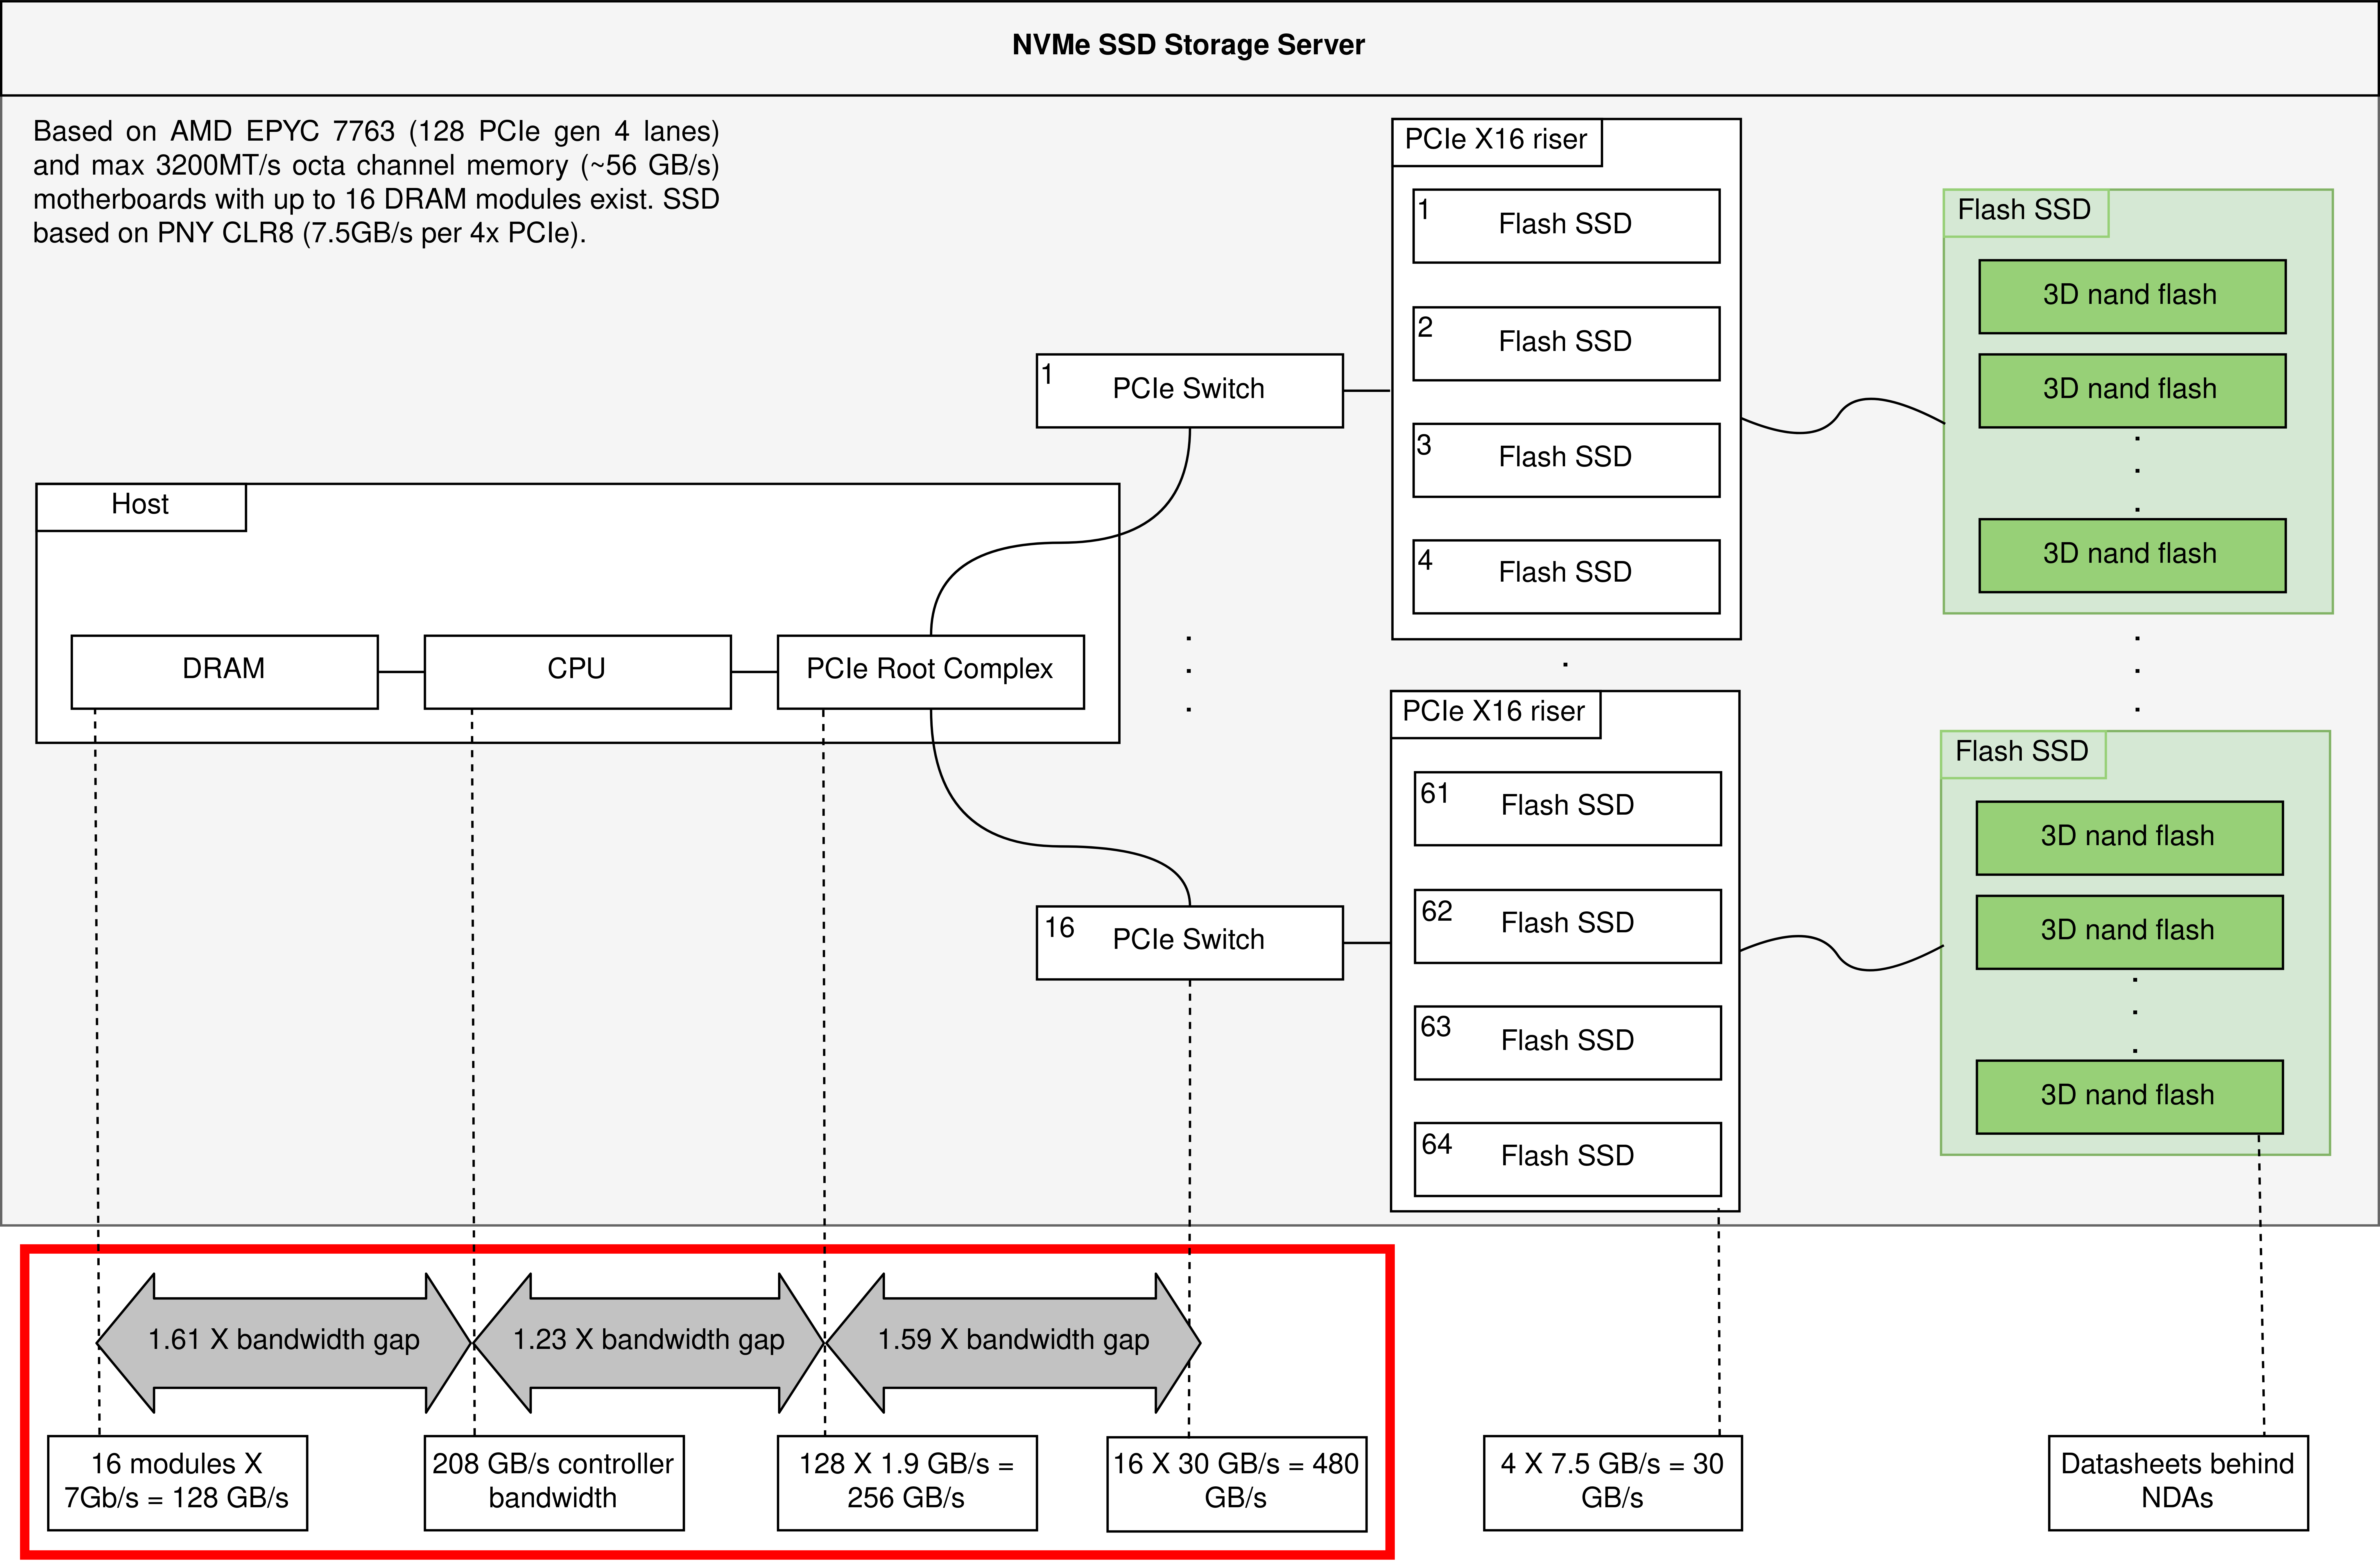
\includegraphics[width=1\textwidth]{resources/images/storage-bottleneck.png}
	\caption{Typical bandwidth limitations in modern storage servers using 64
        SSDs.}
    % \includesvg[width=0.6\columnwidth]{resources/images/module-dependencies}
    \label{figure:storagebottleneck}
\end{figure}

% Potential solution and benefits

A promising solution to this problem is the processing of data in-situ by
pushing compute to the storage layer. This solution is actively being researched
as \textit{"Programmable Storage"} and \textit{"Computational Storage"} among
other terms. The concept is not new however, as it has been previously
explored in database mainframes \cite{database-computer} as well as for
conventional HDDs \cite{active-disk-pillar, active-disks-tech,
intelligent-disk}. With rise of Non-Volatile Memory Express (NVMe) technologies
offering significantly more device-internal bandwidth this concept is being
revised. What makes NVMe SSDs even more suited is that they already contain
capable processing units often boasting even multiple cores. This requirement
comes from the internal management the device has to perform known as the
\textit{Flash Translation Layer} (FTL). Devices utilizing computational elements
on conventional SSDs for \textit{Computational Storage} are commonly known as
\textit{Computational Storage Devices} (CSx)s. The potential benefits of such a
heterogenous architecture offering programmable storage include energy saving,
cost reduction and performance improvements.

% Challenges

Despite all these benefits there is still no widespread adoption even after a
decade of research \cite{lukken2021past}. A multitude of challenges
have prohibited this adoption several are still applicable today. Four
prominent challenges include that, firstly, \textit{Computational Storage}
requires complete vertical integration. Meaning that changes are required at all
levels of abstraction, device hardware, interfaces, drivers and operating system
to name a few. Trying to integrate a solution for all levels in one prototype
results in a very large problem space. This large problem space complicates
deriving standards for designs and interfaces although the development of such a
standard by SNIA is on-going \cite{snia-model}. Secondly, vendors might choose
to use different hardware with different
\textit{Instruction Set Architectures} (ISA)s or different host-to-device
interfaces. These differences might result in incompatible user applications
across vendors hurting reusability and hindering adoption. Third, filesystems
are managed by the host operating system while the FTL is
managed by the device. Given that one is not aware of the processes within the
other, this semantic gap complicates several aspects such as consistency,
concurrency, multi-user tenancy and filesystem integration. Lastly, no
specialized filesystem designs exist that support both regular user access
concurrent with \textit{Computational Storage} offloading.

% Solutions

In this work we address each of these challenges directly and propose a
complete \textit{Computational Storage} solution that offers a filesystem
capable of concurrent multi-user tenancy with both regular and compute
offloading access (hybrid). We introduce each of the solutions briefly before
describing their complete case. Firstly, circumvent the complexity of
complete vertical integration by creating a simulation platform on top of
QEMU \cite{qemu}. Secondly, eliminate potential incompatibilities across
vendors by using \textit{Extended Berkely Packet Filer} (eBPF) \cite{what-ebpf}
as compute kernel language. Third, bridge the semantic gap by using \textit{
Zoned Namespaces} (ZNS) \cite{zns} SSDs which moves the FTL to the host
operating system (host-managed). Lastly, allow for concurrent multi-user
tenancy in a \textit{Hybrid Filesystem} context by developing a specialized
\textit{Log-Structured Filesystem} (LFS) \cite{Rosenblum1992TheDA} with an
in-memory snapshot consistency model \cite{Viotti2016ConsistencyIN}. We present
this complete solution as \textit{OpenCSD} an open-source Apache 2 licensed CSx
simulation framework with accompanying filesystem called
FluffleFS \cite{qemu-csd}.

Clearly computational storage is a promising avenue to the data movement
bottleneck. However, there remain clear challenges that currently prevent it
from being effective. Having mentioned the four parts of our solution briefly we
now describe their complete cases in the next sections.

\subsection{A Case for CSx Simulation}

The lack of a standardized design has lead to a large variety of different
hardware architectures being explored including using embedded CPUs or
\textit{Field-Programmable Gate Arrays} (FPGA)s. Moreover, closed-source
devices have even become commercially available. Still there is a lot of
uncertainty about the right computational hardware models, interconnects and
interconnects their interfaces. Even though the \textit{Peripheral Component
Interconnect Express} (PCIe) interconnect and the NVMe storage interface
currently dominate modern storage devices it is unclear if their current
capabilities are sufficient to support CSxs. Meanwhile existing technologies
such as QEMU allow rapid development of new simulated hardware.

The lack of a clear standardized design combined with the ease of prototyping
designs in simulation clearly shows that choosing simulation over an actual
hardware prototype is the current logical choice.

\subsection{A Case for eBPF Programmability}

The concept of programmability provides end users the capability to run their
own provided code. With the introduction of modern \textit{Operating Systems}
(OS)s this is expected to happen in safe and dynamic manner. Programmability
can be achieved in different manners such as through the kernel in kernel
modules, with filesystems through \textit{Virtual File System} (VFS) or
\textit{Filesystem in USErspace} (FUSE) and with language runtimes such as those
in Python. In addition programmability can also target a peripherals instead of
the host directly such as is prevalent in \textit{General-Purpose computing on
Graphics Processing Units} (GPGPU) programming through \textit{Application
Programming Interfaces} (API)s like OpenCL \cite{opencl} and CUDA \cite{cuda}.
Through similar mechanisms programmability in CSxs can be achieved.

The uncertainty of the hardware design makes it unclear exactly how close to the
hardware and through which method of programmability CSxs will be effective.
Although, naturally, the closer to the actual storage the better
(Near-Data Processing). Therefore, our programmability must not be restricted or
favor a particular type.

Introducing eBPF an ISA and \textit{Application Binary Interface} (ABI) with a
large collection of toolchains and wide-ranging implementations
\cite{what-ebpf, McCanne1993TheBP}. These implementations range from complex,
such as the one found in the Linux kernel, to simple such as the one found in
uBPF \cite{ubpf}, with the key difference in complexity being the supported ABI.
Effectively, the implementation running (runtime) eBPF code decides the ABI by
tying special eBPF syscall instructions to predefined code. In addition, this
allows the user program and runtime to exchange important information such as
prominently done in Linux through eBPF maps \cite{bpf-man}. We demonstrate the
flexibility of such a vendor agnostic ABI as well as the internals of uBPF in
figure \ref{figure:ubpf-abi}.

\begin{figure}
    \centering
	\includegraphics[width=0.8\textwidth]{resources/images/ubpf-abi.pdf}
	\caption{Achieving vendor agnostic \textit{Application Binary Interfaces}
        (ABI) through uBPF.}
    % \includesvg[width=0.6\columnwidth]{resources/images/module-dependencies}
    \label{figure:ubpf-abi}
\end{figure}

The benefits of eBPF are four fold. First, the ISA is not tailored to any
specific domain and it has been used in networking \cite{xdp},
tracing \cite{enhanced-ebpf} and security \cite{seccomp} applications. Second,
the simple nature of the eBPF ISA allows for verification and bounded execution
checking such as performed by the Linux kernel \cite{kern-analysis}. Third, eBPF
supports efficient code generation through jitting achieving close to bare-metal
performance. Lastly, eBPF has been positioned as the unified ISA for
heterogenous computing \cite{Brunella2020hXDPES, bpf-uapi}.

\subsection{A Case for ZNS}

A new emerging NVMe standard is \textit{Zoned Namedspaces} (ZNS). It can been
seen as the technical successor to Open-Channel % \cite{}.
This standard allows host visibility and control over data placement
(host-managed) while more closely representing nand flash behaviour. This
replacement for the traditional block interface offers reduced
write-amplification, lower SSD hardware requirements and more intelligent
wear-levelling and garbage collection. However, ZNS SSDs come with several
constraints such as not allowing in-place updates (append only), using a large
collection of sectors as single erasure unit and requiring wear-levelling and
garbage collection to be explicitly programmed by the host. The fundamental
difference between conventional and ZNS SSDs is shown in figure
\ref{figure:znsvsconventional}.

\begin{figure}
    \centering
	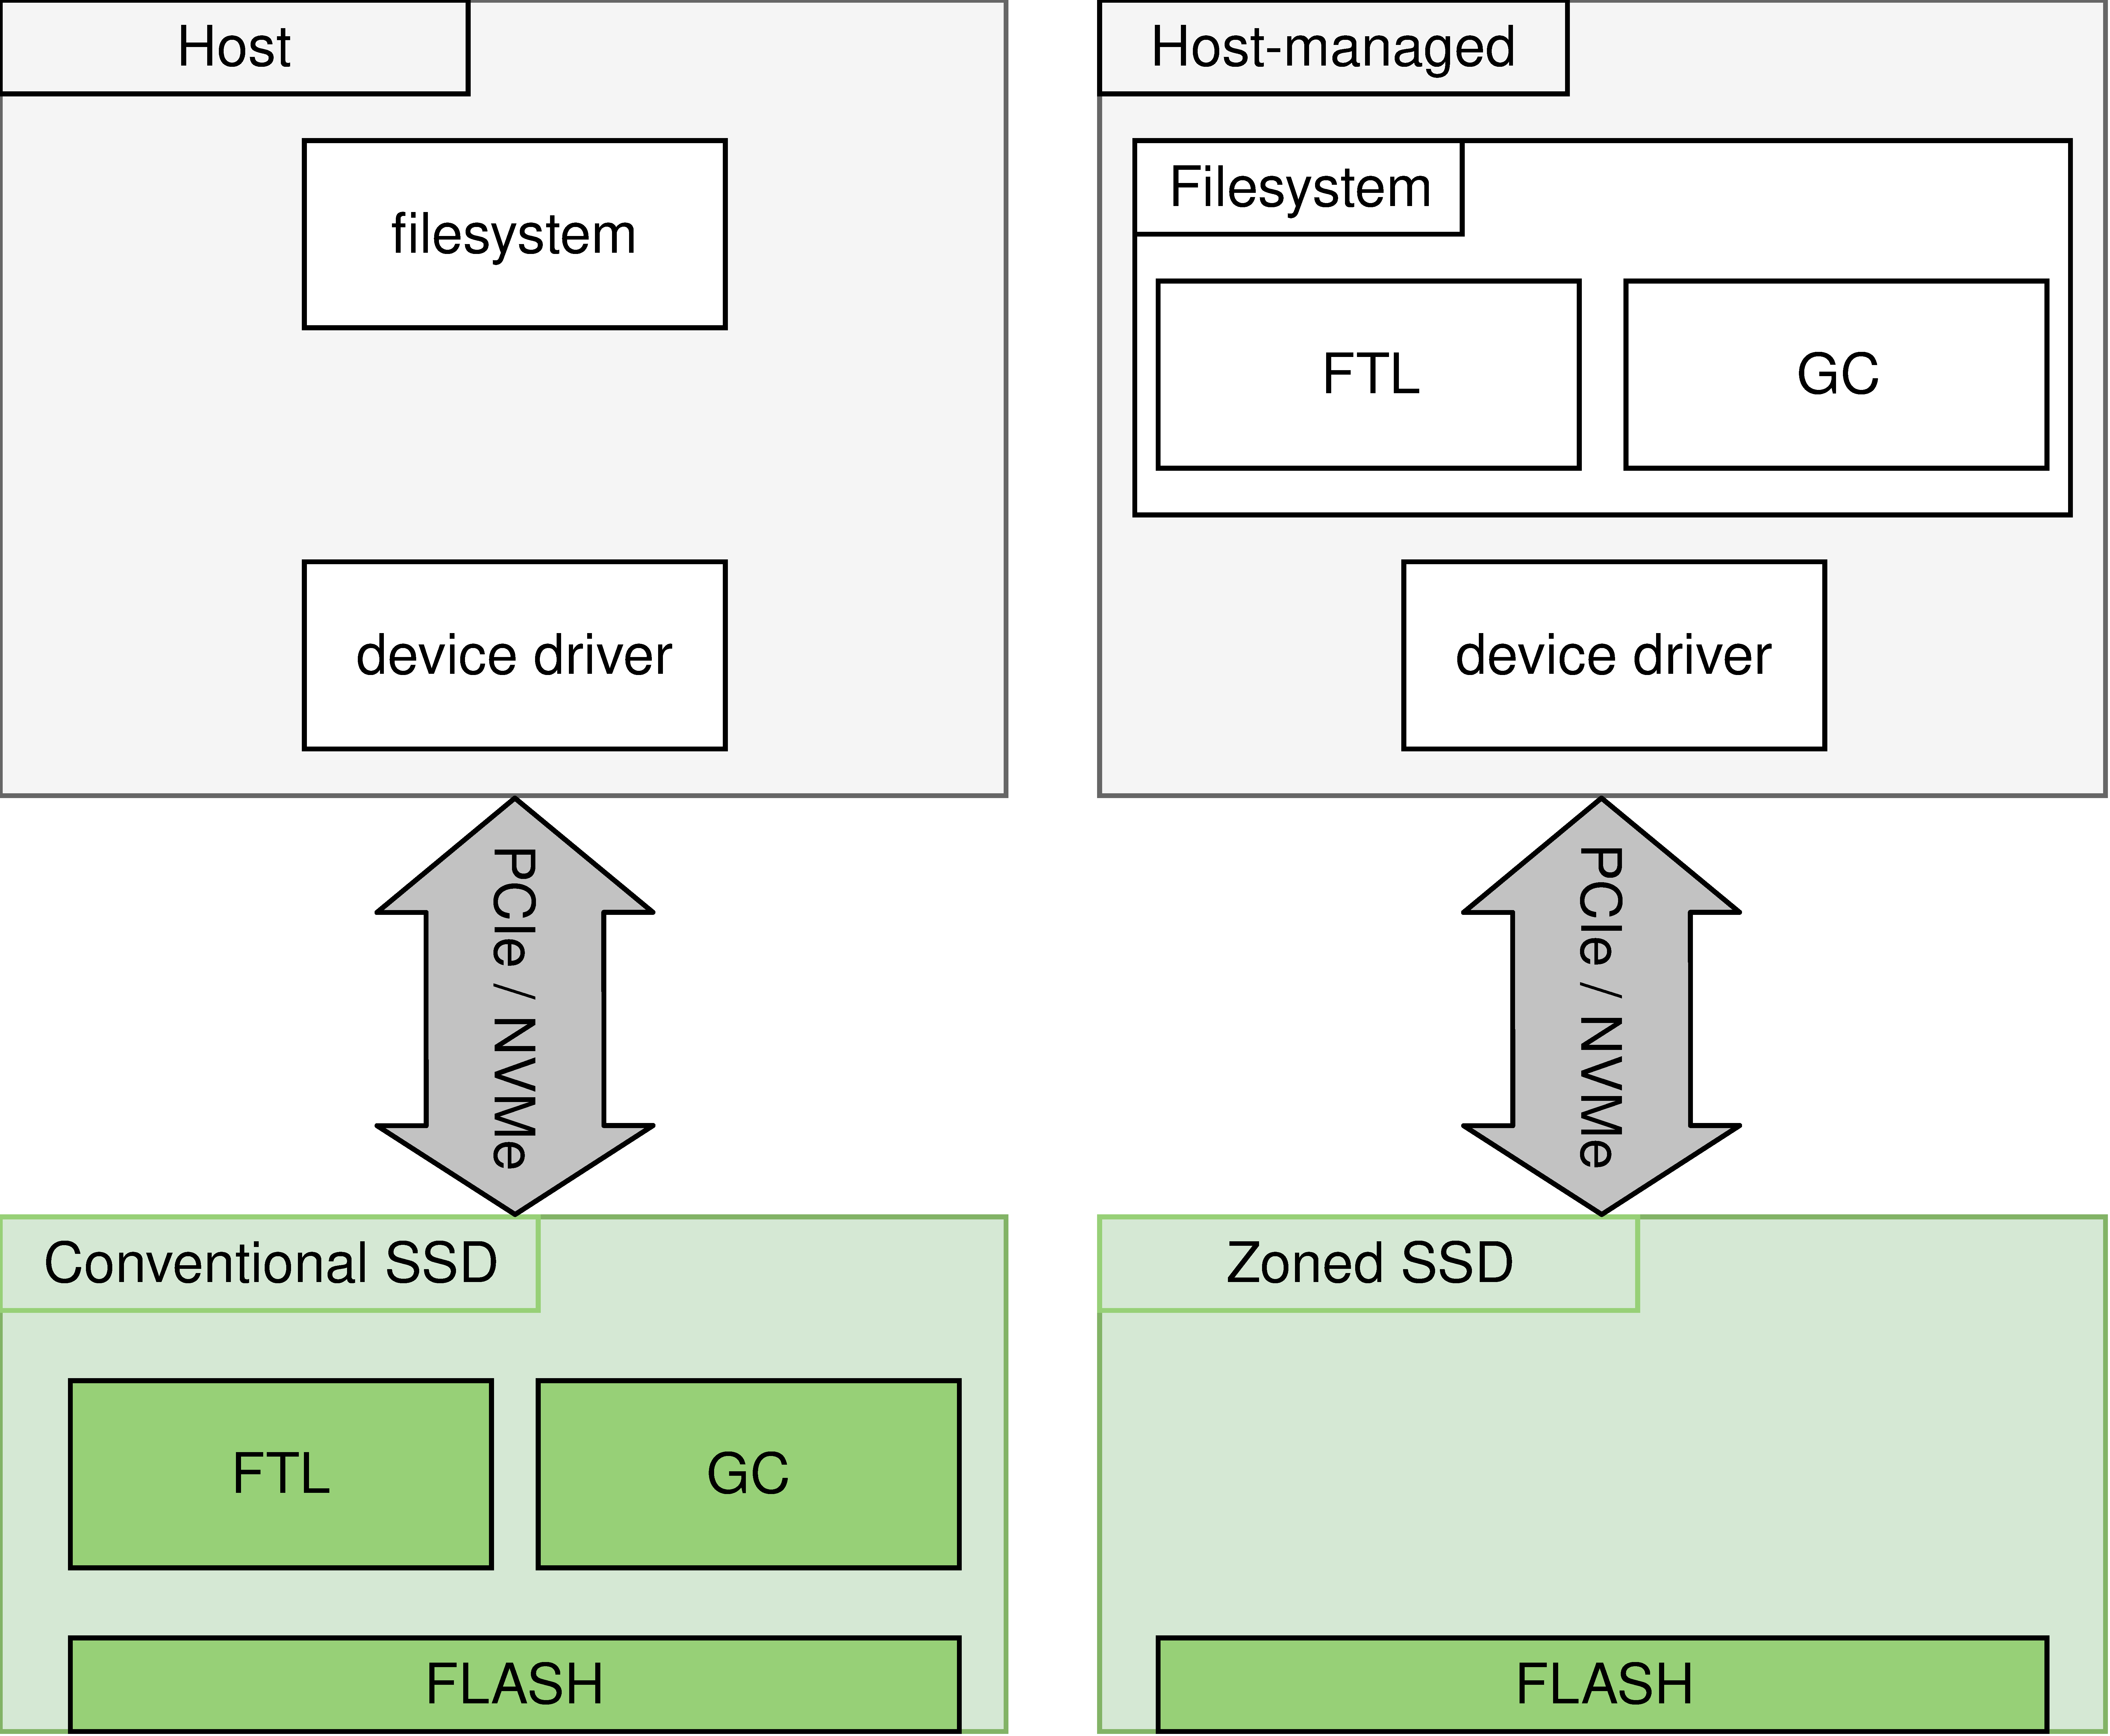
\includegraphics[width=0.6\textwidth]{resources/images/zns-vs-conventional.pdf}
	\caption{Differences between conventional and ZNS SSDs.}
    % \includesvg[width=0.6\columnwidth]{resources/images/module-dependencies}
    \label{figure:znsvsconventional}
\end{figure}

Yet we argue ZNS greatly improves the feasibility of CSx supporting
\textit{hybrid filesystems}. Firstly, ZNS offers more predictable performance in
conjuction with \textit{Log-Structured Filesystems} as the absence of a device
FTL means the behaviour of \textit{append-only} writes won't be influenced by
underlying write-amplification or garbage-collection. Secondly, the direct
relationship between dimensions as reported to the host and to those known on
the device results in a greatly simplified exchange of information from host
submitted compute kernels as well as reduced kernel runtime translations.
Finally, this reduced semantic gap between the host and device is essential to
compute kernels running autonomously and without shared virtual memory.

\subsection{A Case for LFS}

\textit{Log-Structured Filesystems} have been around for a long
time \cite{Rosenblum1992TheDA} but have not really been popularized until the
recent advancement of nand flash. A LFS maintains one or multiple logs which
are append only sections of the filesystem. This has the advantage of the
underlying device receiving filesystem writes as sequential I/O operations,
which is known to improve performance. In addition, LFSs are often relatively
easy to implement. Unfortunately, LFSs suffer from write-amplification because
modifications updating inode or other data location information travels up the
chain in history. The specific type of write-amplification common in LFSs is
also known as the wandering tree problem. An example of write-amplification is
shown in figure \ref{figure:writeamplification}.

\begin{figure}
    \centering
	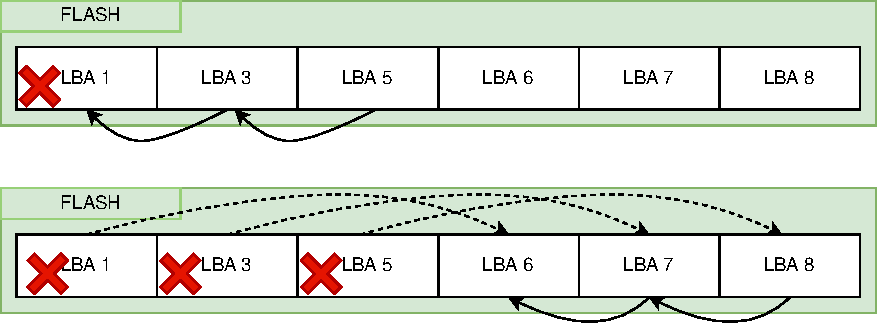
\includegraphics[width=0.7\textwidth]{resources/images/write-amplification.pdf}
	\caption{Example of write-amplification where a single invalidation leads
    to multiple linked blocks being rewritten.}
    % \includesvg[width=0.6\columnwidth]{resources/images/module-dependencies}
    \label{figure:writeamplification}
\end{figure}

Yet we argue an LFS is essential for an effective \textit{hybrid filesystem} due
to the following three reasons. Firstly, the append-only nature of a LFS is the
best fit for the append-only requirement of ZNS SSDs. Secondly, the
chronological order of logs allows for snapshotting, versioning and simplified
crash recovery. It is thanks to the properties of an LFS that FluffleFS is able
to provide in-memory snapshots to compute kernels. Lastly, the problem around
write-amplification is a solved issue thanks to the F2FS \cite{Lee2015F2FSAN}
work which introduced a so called \textit{Node Address Table} (NAT). A diagram
showing a simplified view of F2FS and the NAT is shown in figure
\ref{figure:f2fsnat}.

\begin{figure}
    \centering
	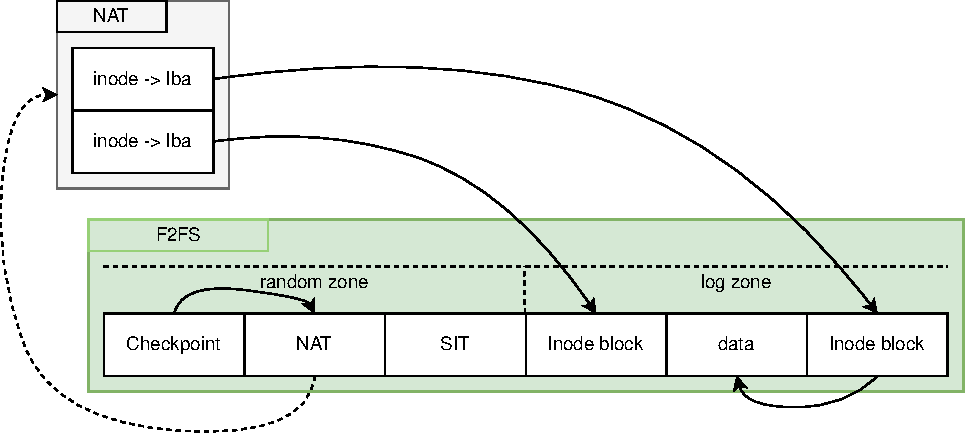
\includegraphics[width=0.7\textwidth]{resources/images/f2fs-nat.pdf}
	\caption{Overcoming LFS limitations with a separate random zone and NAT.}
    % \includesvg[width=0.6\columnwidth]{resources/images/module-dependencies}
    \label{figure:f2fsnat}
\end{figure}

As shown each of these cases demonstrates the importance of each part. Only
together are they able to provide a complete solution for open research
questions given the current state of the field as we will proof in the design
section.

\section{Research Question}

The main scientific contribution of this work is formulated in the form of a
research question. In addition, we formulate several sub questions which aid in
showing to which extend the main research question is answered. The sub research
questions relate both to design choices as well as qualitative performance
evaluations.

Our main scientific contribution aims to answer one of the most prominent open
research questions in the field of Computational Storage. The question of
designing a filesystem that supports both regular and offloaded access, so
called \textit{hybrid filesystems}. We formulate that into the following
research question. Namely,

\begin{displayquote}
    How to create a multi-user tenant (hybrid) LFS with Computational Storage
    offloading support?
\end{displayquote}

\subsection{Sub Questions}

% Ensure the research questions are such that they support the design
% requirements.

\begin{itemize}
    \item Design Requirements
    \begin{enumerate}
        \item What existing technologies are best suited for a hybrid LFS?
        \item What techniques can be used to minimize the complexity required to
              use a hybrid LFS?
        \item What mechanisms allow for simplified replacement of used existing
              technologies in a hybrid LFS?
        \item How to register CSx compute kernels using existing operating 
              system APIs?
        \item How to differentiate individual users, files and I/O operations in
              relation to their CSx compute kernel?
        \item How to design a compute kernel API that can be reused across
              devices?
        \item How to ensure user submitted CSx compute kernels are safe?
    \end{enumerate}
    \item Experimental Evaluation
    \begin{enumerate}
        \item Can a multi-user tenant hybrid LFS achieve unstagnated performance
              for concurrent regular and offloaded file access?
        \item Can a multi-user tenant hybrid LFS reduce the data movement
              between device and host?
        \item Can a multi-user tenant hybrid LFS reduce the host load for
              asynchronous applications?
    \end{enumerate}
\end{itemize}

Our design requirements aim to result in practical solution that can easily be
adopted should new technologies emerge with high ease of use while actually
allowing for concurrent regular and offloaded access. In addition, our
experimental evaluation aims to show that while doing so we can achieve the
expected benefits of such designs.

\section{Research Method}

A well-defined research method is needed to answer the main, design requirements
and performance evaluation research questions. Given the nature of the work,
being the development and evaluation of a research software prototype, an
iterative design approach similar to that of Agile is best suited. Meanwhile the
evaluation method uses a more straightforward approach consisting of several
performance evaluations. Each of these evaluations provides evidence supporting
claims made about the multi-user tenant hybrid LFS.

Given the large of possible iterative design approaches we describe ours
more elaborately in the next section.

\subsection{Design Approach}

Our design approach consists of an initial step performed only once followed by
as many iterations as necessary to complete the design. The first being
identifying the critical components. Subsequently, the iterative design approach
consists of the following three steps. First, identify existing technologies
that can be used for one or more of the critical components. Secondly,
evaluate each of the potential technologies. Third, implement the
functionality of the component using the selected technology. Any issue that
prevents the further use of a chosen technology starts the next iteration of the
design process. If no alternatives can be found workarounds or practical
limitations are introduced instead.

This design approach should allow for the selection of the best available
existing technologies given the design requirements while allowing to change
any chosen technologies during the implementation process.
